%	\begin{itemize}
%	\item \justifying \textbf{\textit{Recurso}} es cualquier \textit{persona, lugar, documento, p�gina web, objeto abstracto o f�sico} que tiene un identificador �nico de recursos (URI). \\ Por ejemplo, UAM $=>$ \url{http://www.mi-ejemplo.com/UAM} 
%	\item \justifying \textbf{\textit{Propiedad}} es un aspecto significativo, caracter�stica, o relaci�n que se describe de un recurso.
%	\begin{itemize}
%		\item Propiedad Objeto: describe una relaci�n entre dos recursos.
%		\item Propiedad Objeto: describe una relaci�n entre un objeto y una literal (cadena, entero, flotante, fecha).
%	\end{itemize}	
%	Por ejemplo, nombre $=>$ \url{http://www.mi-ejemplo.com/tiene-nombre} 
%	\item \justifying \textbf{\textit{Declaraci�n}} es una afirmaci�n de un hecho expl�cito de un recurso, en t�rminos de una propiedad y el valor asignado a �sta (otro recurso o literal). La forma b�sica para escribir una declaraci�n, es la \textbf{\textit{tripleta}} \cite{SemWebTim}.
%	\begin{enumerate}
%	\item \textbf{\textit{Sujeto}} es el recurso que se describe.
%	\item \textbf{\textit{Predicado}} es la propiedad.
%	\item \textbf{\textit{Objeto}} es otro recurso o una literal (cadena o entero) que describe el predicado.
%	\end{enumerate}
%	\end{itemize}

%	\begin{block}{Naturaleza en los Recursos de Informaci�n}
%		\begin{itemize}
%		\item Diversidad en el Formato:\\ \textit{pdf, doc, odp, html, txt, xsl, wav, png, mp3, mp4, mpeg, mov, ppt, flv, por mencionar algunas}.
%		\item Diversidad en el Contenido:\\ \textit{p2p, middleware, estado global, sistema operativo, replicaci�n, concurrencia, sincronizaci�n, entre otras}.
%		\item Diversidad en la Estructura:\\ \textit{datos estructurados, semi-estructurados y sin estructura}.
%		\item Significado de la Informaci�n
%			\begin{itemize}
%			\item Homonimia: \textbf{radio} tiene distintos significados que se asocian a la Qu�mica, Comunicaci�n, Anatom�a o Geometr�a.
%			\item Sinonimia: \textbf{resumen}, \textbf{sumario}, \textbf{s�ntesis} y \textbf{recapitulaci�n}.
%			\end{itemize}
%		\end{itemize}
%	\end{block}

%	\begin{block}{Objetivos de una ontolog�a}
%	\begin{enumerate}
%	\item \justifying Construir un vocabulario conceptual, formal y consensuado para un dominio dado.
%	\item \justifying Inferir informaci�n a partir de un conjunto de reglas y hechos que descri
%	
%	, as� como para componer expresiones complejas en el vocabulario.
%	\item \justifying Un vocabulario para construir descripciones y comunicar hechos.
%	\item \justifying Interpreten sin ambig�edad el conocimiento y vocabulario de un dominio dado.
%	\item \justifying Intercambiar y reutilizar el conocimiento para diferentes prop�sitos.
%	\item \justifying Inferir informaci�n a partir de un programa especializado (razonador) y los hechos en una ontolog�a.
%	\end{enumerate}
%	\end{block}


%\subsubsection{Resource Description Framework (RDF)}
%\begin{frame}[allowframebreaks]
%	\frametitle{Resource Description Framework (RDF)}
%	%%%%%%%%%%%%%%%%%%%%%%%%%%%%
%	
%	
%	
%	%%%%%%%%%%%%%%%%%%%%%%%%%%%%
%	
%	
%\end{frame}
%
%\subsubsection{SPARQL}
%\begin{frame}[allowframebreaks]
%	\frametitle{SPARQL}
%	\begin{block}{Definici�n}
%	\justifying 
%	Lenguaje de consulta y protocolo de acceso a RDF, para la b�squeda y recuperaci�n de la informaci�n en un grafo RDF.
%	\end{block}
%	
%	\begin{figure}
%	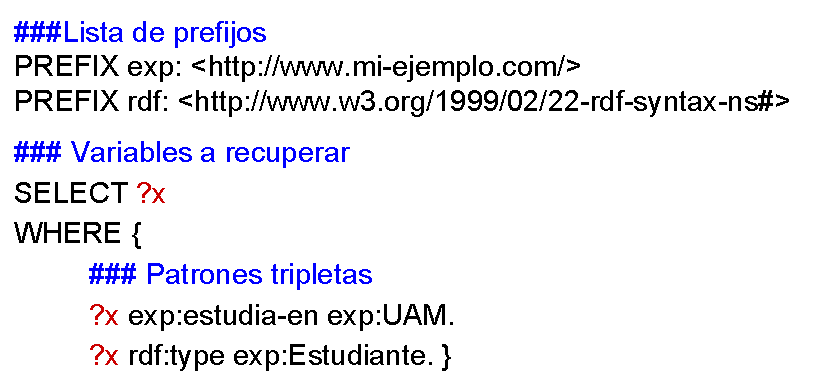
\includegraphics[scale=0.52]{FormaSPARQL} 
%	\end{figure}
%\end{frame}
%
%
%
%\subsubsection{Inferencia}
%\begin{frame}
%	\frametitle{Inferencia}
%	\begin{block}{Razonador}
%	Un programa que deduce declaraciones a partir de los axiomas y declaraciones expl�citas en la ontolog�a.
%	\end{block} 
%	
%	\begin{figure}
%	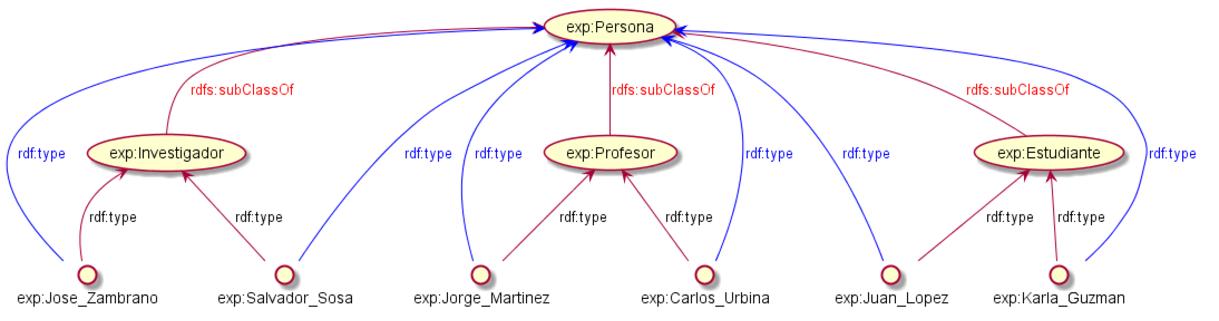
\includegraphics[scale=0.52]{grafoInfBasico} 
%	\end{figure}
%\end{frame}